\linespread{1.1}         			% Palatino needs more leading (space between lines)
\chapter{Pr�sentation de l'entreprise et contexte g�n�ral du projet }
%%%%%%%%%%%%%%%%%%%%%%%%%%%%%%%%%%%%%%%%%%%%%%%%%%%%%%%%%%%%%%%%%%%%%
\label{Chapitre-1}
\minitoc
\linespread{1.2}         			% Palatino needs more leading (space between lines)
\newpage

\section{Introduction}
%%%%%%%%%%%%%%%%%%%%%%%
\noindent En r�sum�, ...
\begin{itemize}
	\item	Pr�senter l'entreprise d'acceuil ;
	\item	Contexte du projet : cadre du projet, objectifs du projet, diagramme de GANTT ;
	\item etc.\\
\end{itemize}

Dans la suite de ce chapitre, nous allons utiliser diverses caract�ristiques de LaTeX. \\

\section{Pr�sentation de l'organisme d'acceuil} 
%%%%%%%%%%%%%%%%%%%%%%%%%%%%%%%%%%%%%%%%%%%%%%%

\subsection{Mission de l'entreprise}
%-----------------------------------

\subsubsection{En gras}
\textbf{Ceci est un texte en gras}.\\

\subsubsection{En italique}
\textit{Ceci est un texte en italique}.\\

\subsubsection{En Soulign�}
\underline{Ceci est un Texte soulign�}.\\

\subsubsection{R�f�rence dans le bas de page}
Ceci est un texte r�f�renc� dans le bas de page\footnote{Explications en bas de page}.\\

\subsubsection{Entre parenth�se}
(Ceci est un texte entre parenth�ses).\\

\subsubsection{Entre guillemet}
\og Ceci est un texte entre guillemet \fg{}.\\

\subsubsection{Texte en petites capitales}
\textsc{Ceci est un texte en petites capitales}.\\

\subsubsection{Pour aller plus loin ...}
\noindent Pour plus de commandes sur LaTex, vous pouvez acc�der au site : https://www.xm1math.net/doculatex/\\

\subsection{Organigramme}
%-----------------------
Voila un exemple, pour afficher une image dans la figure \ref{fig:fonctions-�valuation}. Cette image provient de la r�f�rence bibliographique \cite{Hadji2000} et se trouve dans le r�pertoire "images" de ce projet LaTeX :

\begin{figure}[h]
	\centering
	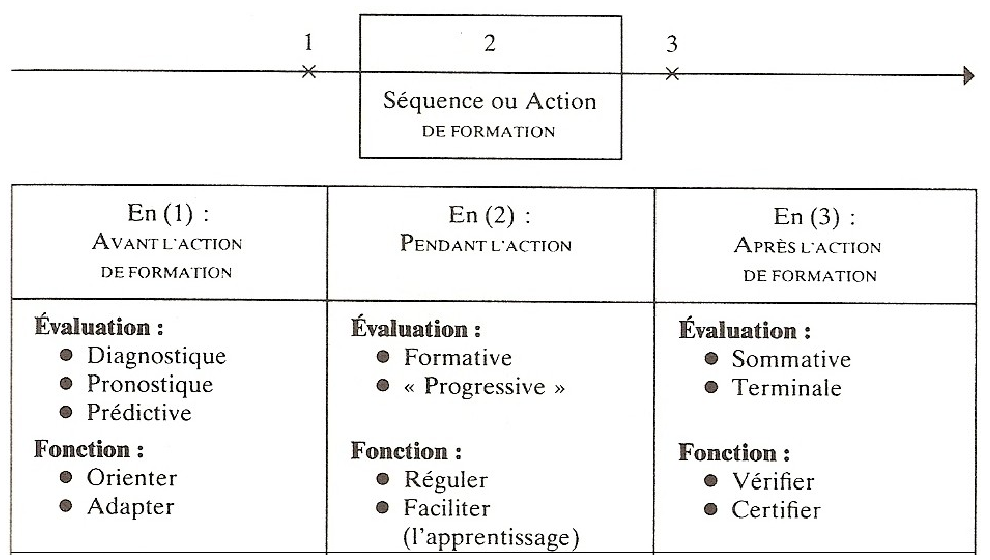
\includegraphics[scale=0.50]{images/types-evaluations.pdf}
	\caption{Fonctions de l'�valuation selon sa place par rapport � l'action de formation \cite{Hadji2000}}
	\label{fig:fonctions-�valuation}
\end{figure}

\subsection{...}
%--------------

\section{Contexte du projet}
%%%%%%%%%%%%%%%%%%%%%%%%%%%%
\subsection{Cadre du projet}
%---------------------------
\noindent Ceci est une ligne qui ne commence pas par une tabulation. \\ 

\subsection{Objectifs du projet}
%-------------------------------
\noindent Ceci est une liste num�rot�e :
\begin{enumerate}
	\item	Ligne 1 ... ;
	\item	Ligne 2 ... ;
	\item	Ligne 3 ... ;
	\item	Ligne 4 ... ;
	\item	Ligne 5 ... ;
	\item	Ligne 6 ... .	\\
\end{enumerate}

\subsection{Diagramme de GANTT}
%---------------------------
\noindent Ceci est une liste avec des puces :
\begin{itemize}
	\item	Ligne 1 ... ;
	\item	Ligne 2 ... ;
	\item	Ligne 3 ... ;
	\item	Ligne 4 ... ;
	\item	Ligne 5 ... ;
	\item	Ligne 6 ... .	\\
\end{itemize}

\subsection{...}
%---------------


\section{Conclusion}
%%%%%%%%%%%%%%%%%%%


   













